\usetikzlibrary{arrows.meta}
\tikzset{
  exam conic edge/.style={line width=.6pt},
  exam conic curve/.style={line width=.6pt},
  exam conic axis/.style={line width=.6pt,>=Stealth},
  exam conic label/.style={inner sep=0pt,outer sep=0pt,font=\normalsize}
}
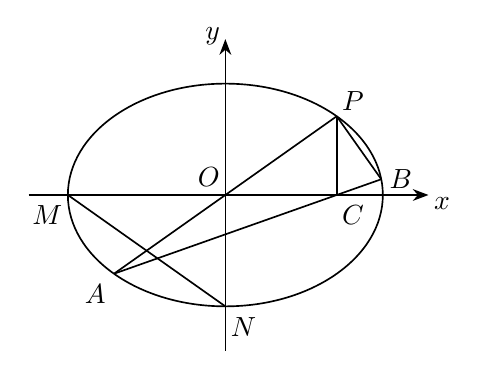
\begin{tikzpicture}[x=1cm,y=1cm,line width=.6pt,font=\normalsize,>=Stealth]
\coordinate (O) at (0,0);
\coordinate (M) at (-2,0);
\coordinate (N) at (0,-1.414213562);
\coordinate (P) at (1.414213562,1);
\coordinate (A) at (-1.414213562,-1);
\coordinate (C) at (1.414213562,0);
\coordinate (B) at (1.979898987,0.2);
\coordinate (Xleft) at (-2.5,0);
\coordinate (Xright) at (2.58,0);
\coordinate (Ydown) at (0,-1.98);
\coordinate (Yup) at (0,1.98);
\draw[exam conic curve] (O) ellipse [x radius=2cm, y radius=1.414213562cm];
\draw[exam conic edge] (M)--(N);
\draw[exam conic edge] (A)--(P);
\draw[exam conic edge] (P)--(C);
\draw[exam conic edge] (A)--(B);
\draw[exam conic edge] (P)--(B);
\draw[exam conic axis,->] (Xleft)--(Xright);
\draw[exam conic axis,->] (Ydown)--(Yup);
\node[exam conic label,below left,xshift=-2pt,yshift=-4pt] at (M) {$M$};
\node[exam conic label,below right,xshift=2pt,yshift=-4pt] at (N) {$N$};
\node[exam conic label,above right,xshift=2pt,yshift=2pt] at (P) {$P$};
\node[exam conic label,below left,xshift=-3pt,yshift=-4pt] at (A) {$A$};
\node[exam conic label,right,xshift=3pt] at (B) {$B$};
\node[exam conic label,below right,xshift=2pt,yshift=-4pt] at (C) {$C$};
\node[exam conic label,above left,xshift=-2pt,yshift=3pt] at (O) {$O$};
\node[exam conic label,below right,xshift=2pt,yshift=-1pt] at (Xright) {$x$};
\node[exam conic label,left,xshift=-2pt,yshift=1pt] at (Yup) {$y$};
\end{tikzpicture}
